\section{Improving throughput by changing buffer size} \label{sec:improving_throughput}

In previous test \label{sec:delay_on_links} we saw that using the same bandwith but introducing high delay on links decrease the throughput significantly.
This is likely to be due to wrong buffer size more precisely TCP window size.
In this section we will try to adjust buffer size and see if it improves  the results.
I will only use TCP as the OpenVPN protocol because UDP is not my main focus here.

To adjust the TCP maximum send and receive window size, I will set value of \textit{sndbuf} and \textit{rcvbuf} in the openvpn configuration.
To compute the size I will be using the formula : $$(2 * delay * bandwidth) * 2$$.

First I will try on one specific setup from test \ref{sec:delay_on_links}, the 8mbit/s bandwidth limit and 400 RTT.

Now lets use a buffer size of 800000 bytes (390 kbytes) instead of the default one used by openvpn (64kbytes)

This is done by modifying the openvpn configuration file of client and server see \ref{lst:set_buffer_size_openvpn}:

  \begin{lstlisting}[caption={Set buffer size OpenVPN configuration},label={lst:set_buffer_size_openvpn}]
	proto tcp
	sndbuf 800000
	rcvbuf 800000\end{lstlisting}

And modify the maximum buffer size that applications can request by changing /proc/sys/net/core/rmem\_max and /proc/sys/net/core/wmem\_max on the onpenvpn client and
openvpn server~\cite{tcptuning}. You might also have to change the /proc/sys/net/ipv4/tcp\_wmem and /proc/sys/net/ipv4/tcp\_rmem if they are not big enough.(see \ref{lst:set_buffer_size_os})

\begin{lstlisting}[caption={Set max buffer size},label={lst:set_buffer_size_os}]
sysctl -w net.core.wmem_max=800000
sysctl -w net.core.rmem_max=800000
sysctl -w net.ipv4.tcp_rmem='4096	87380	6291456'
sysctl -w net.ipv4.tcp_wmem='4096 16384	4194304'\end{lstlisting}

This gives a 10mbit/s throughput and an average RTT of 450 (see figure \ref{tcp_all_custom_buffer}). This is obviously a better result than the 2mbit/s throughput seen on figure \ref{tcp_vs_udp_200ms}.

  \begin{figure}[h!]
    \centering
    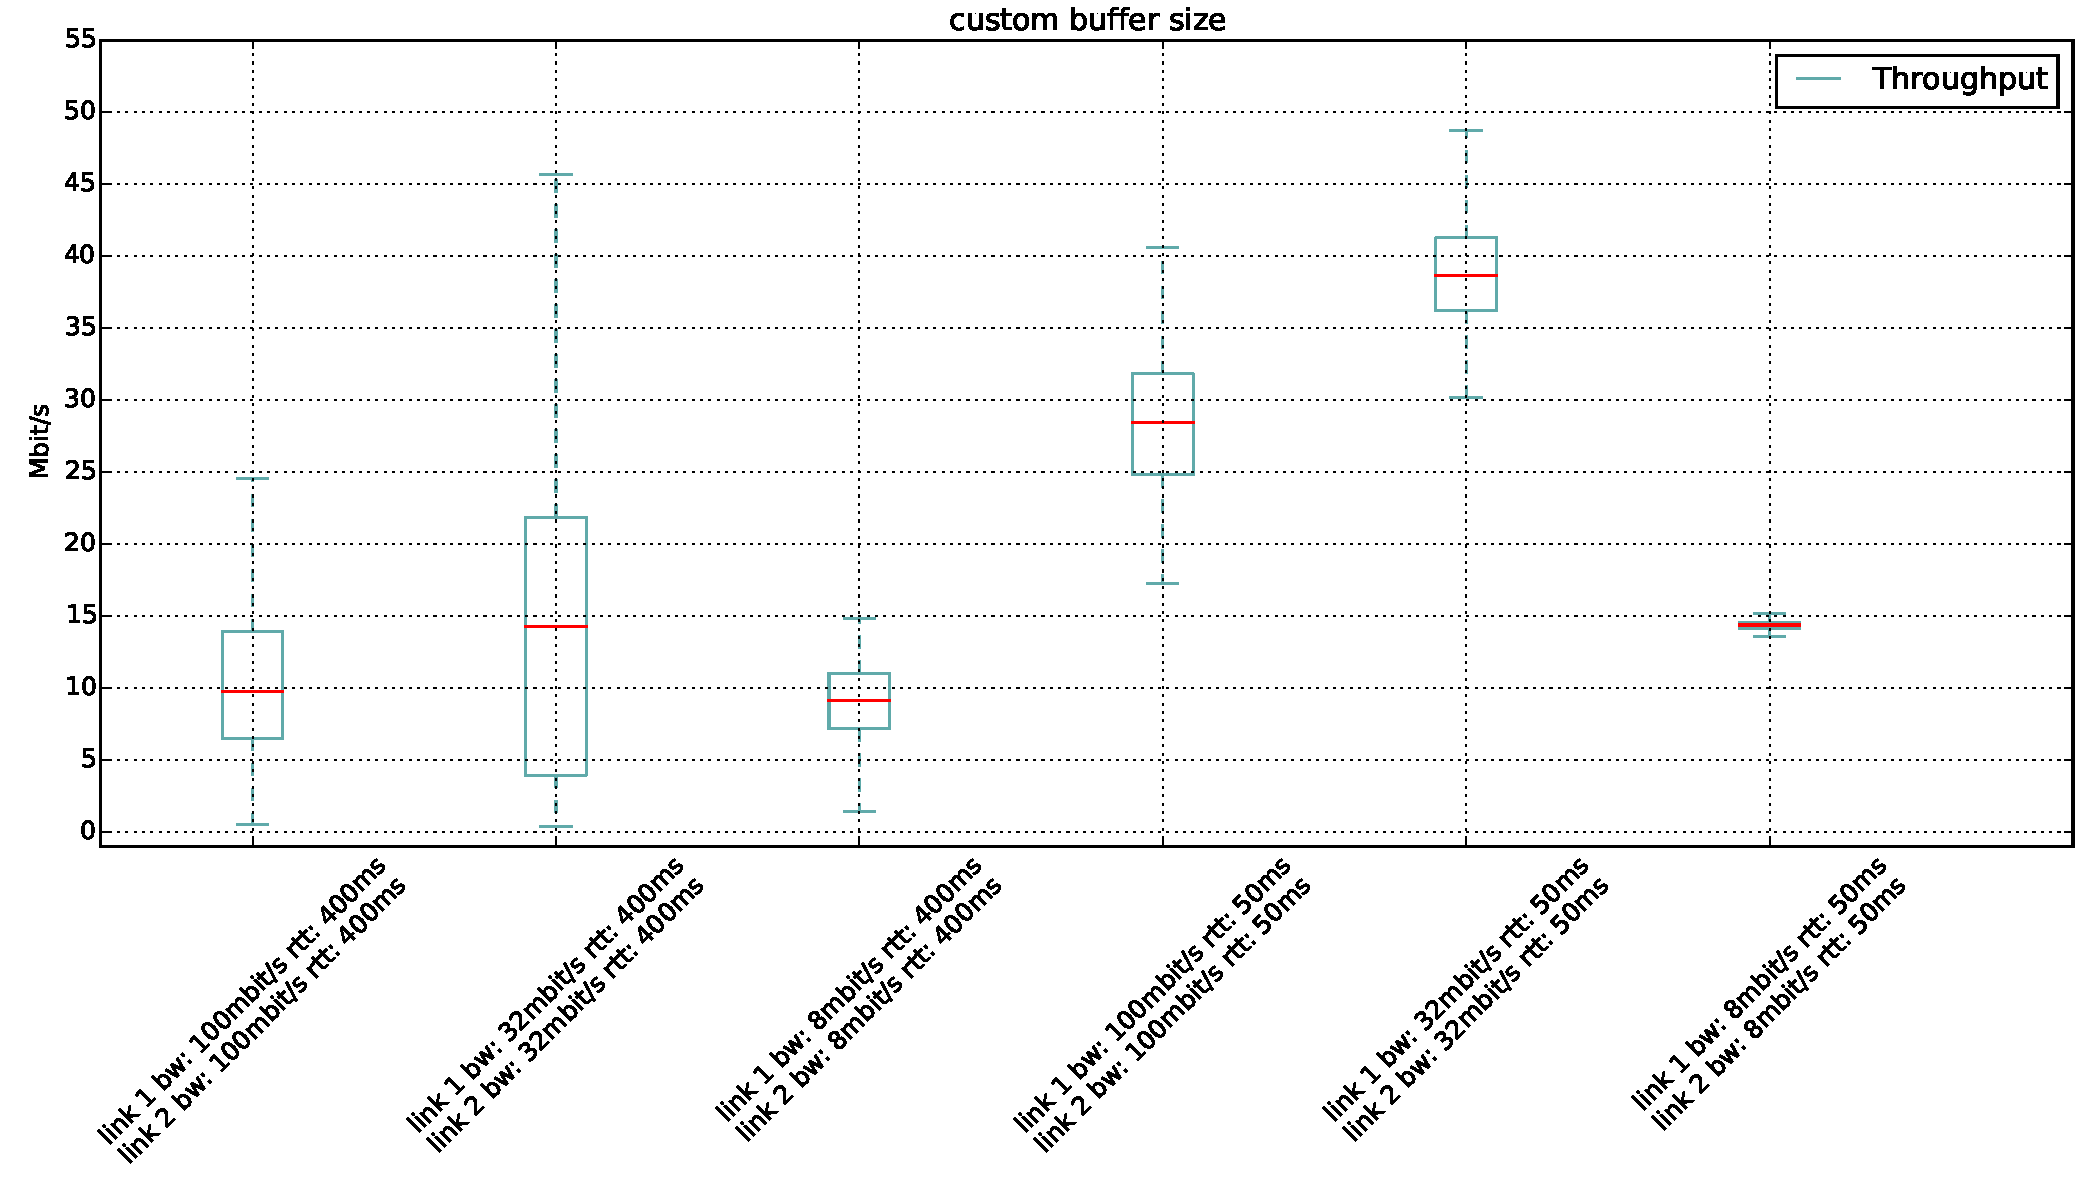
\includegraphics[width=1\textwidth]{../results/tcp_all_custom_buffer.pdf}
    \caption{TCP custom buffer size}
    \label{tcp_all_custom_buffer}
  \end{figure}

On figure \ref{tcp_all_custom_buffer} the same technique is applied for 32mbit/s and 100mbit/s.
It is interesting to see that it improves the throughput in every cases but it does not equal the results obtained with a 2ms RTT.
I tried many different buffer sizes but I was unable to match it.

There is also some unexpected results like the 100mbit/s links with a RTT of 50 only giving a throughput around 30 mbit/s. To but sure I have looked at the sender window but
it did not fill the receiver window, this was not the problem. Analysing the capture with MPTCPTrace I saw on the sequence graph some \"flat\" increase
suggesting that packet losses were happening. Using TCPTrace I looked at the encapsulated connection and indeed there was some packet losses which could be the reason for the
window not to increase.

Looking at the packet capture I determined that the higher RTT, the more retransmissions were occurring which implies a decrease in the throughput.

Another very interesting thing is that the retransmissions happens only in the encapsulated TCP connection. Because TCP over TCP is used, there is a upper layer
which is the OpenVPN packet supporting MPTCP and a lower layer, which is the traffic from the computer client with normal TCP encapsulated in the upper layer.

The retransmission could happen in both layers but here we observe that it only happens in the lower layer.
This is positive in the sense that it does not retransmit multiple times on the different layers, meaning that it does not have the TCP meltdown effect~\cite{tcpovertcp}.
This also tell us that the upper layer, the MPTCP connection is limited by the lower layer.

This is illustrated in figure \ref{upper_seq} and figure \ref{lower_seq}.
Figure \ref{upper_seq} shows the sequence graph generated with MPTCP on the upper layer TCP connection, it shows that the line is pretty flat between time 105 and 120.
Figure \ref{lower_seq} shows the sequence graph generated by TCPTrace on the lower layer TCP connection at time 105. On this figure a lot of SACK and some retransmissions are observable meaning
that there is packet losses at this time.

\begin{figure}[h!]
  \centering
  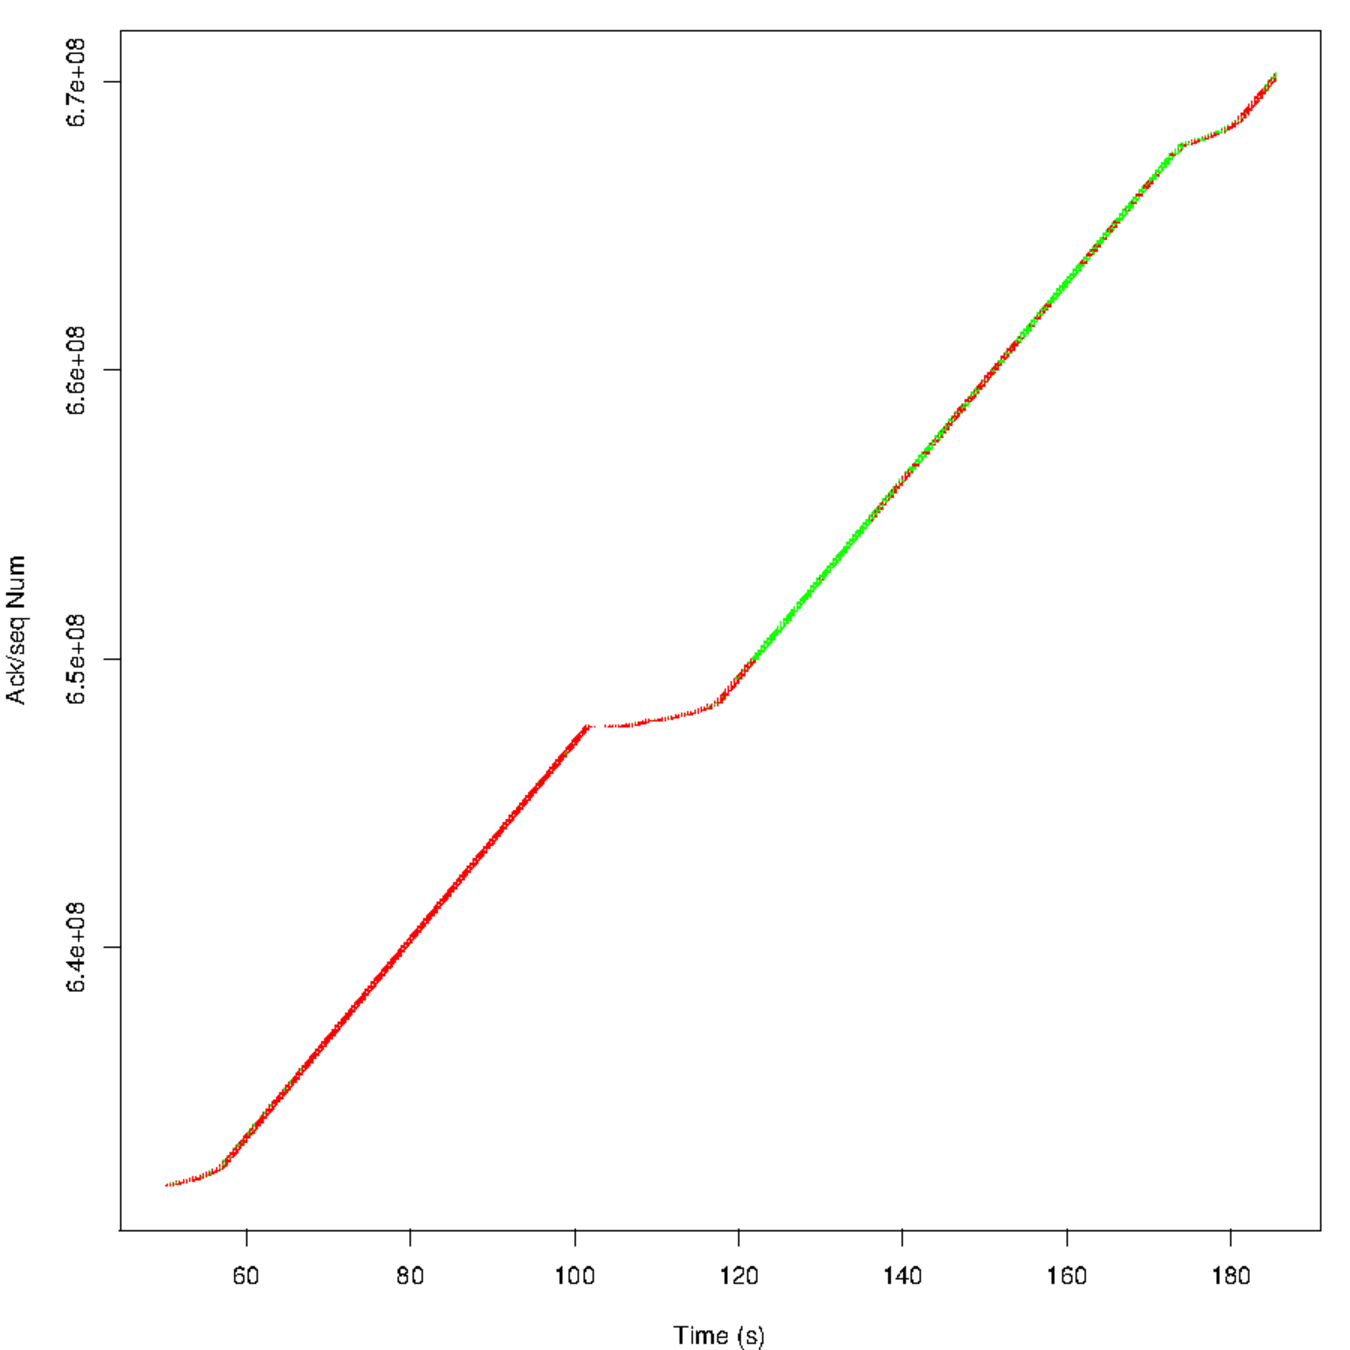
\includegraphics[width=10cm]{../results/upper_layer_seq.pdf}
  \caption{Sequence graph of the upper layer}
  \label{upper_seq}
\end{figure}

\begin{figure}[h!]
  \centering
  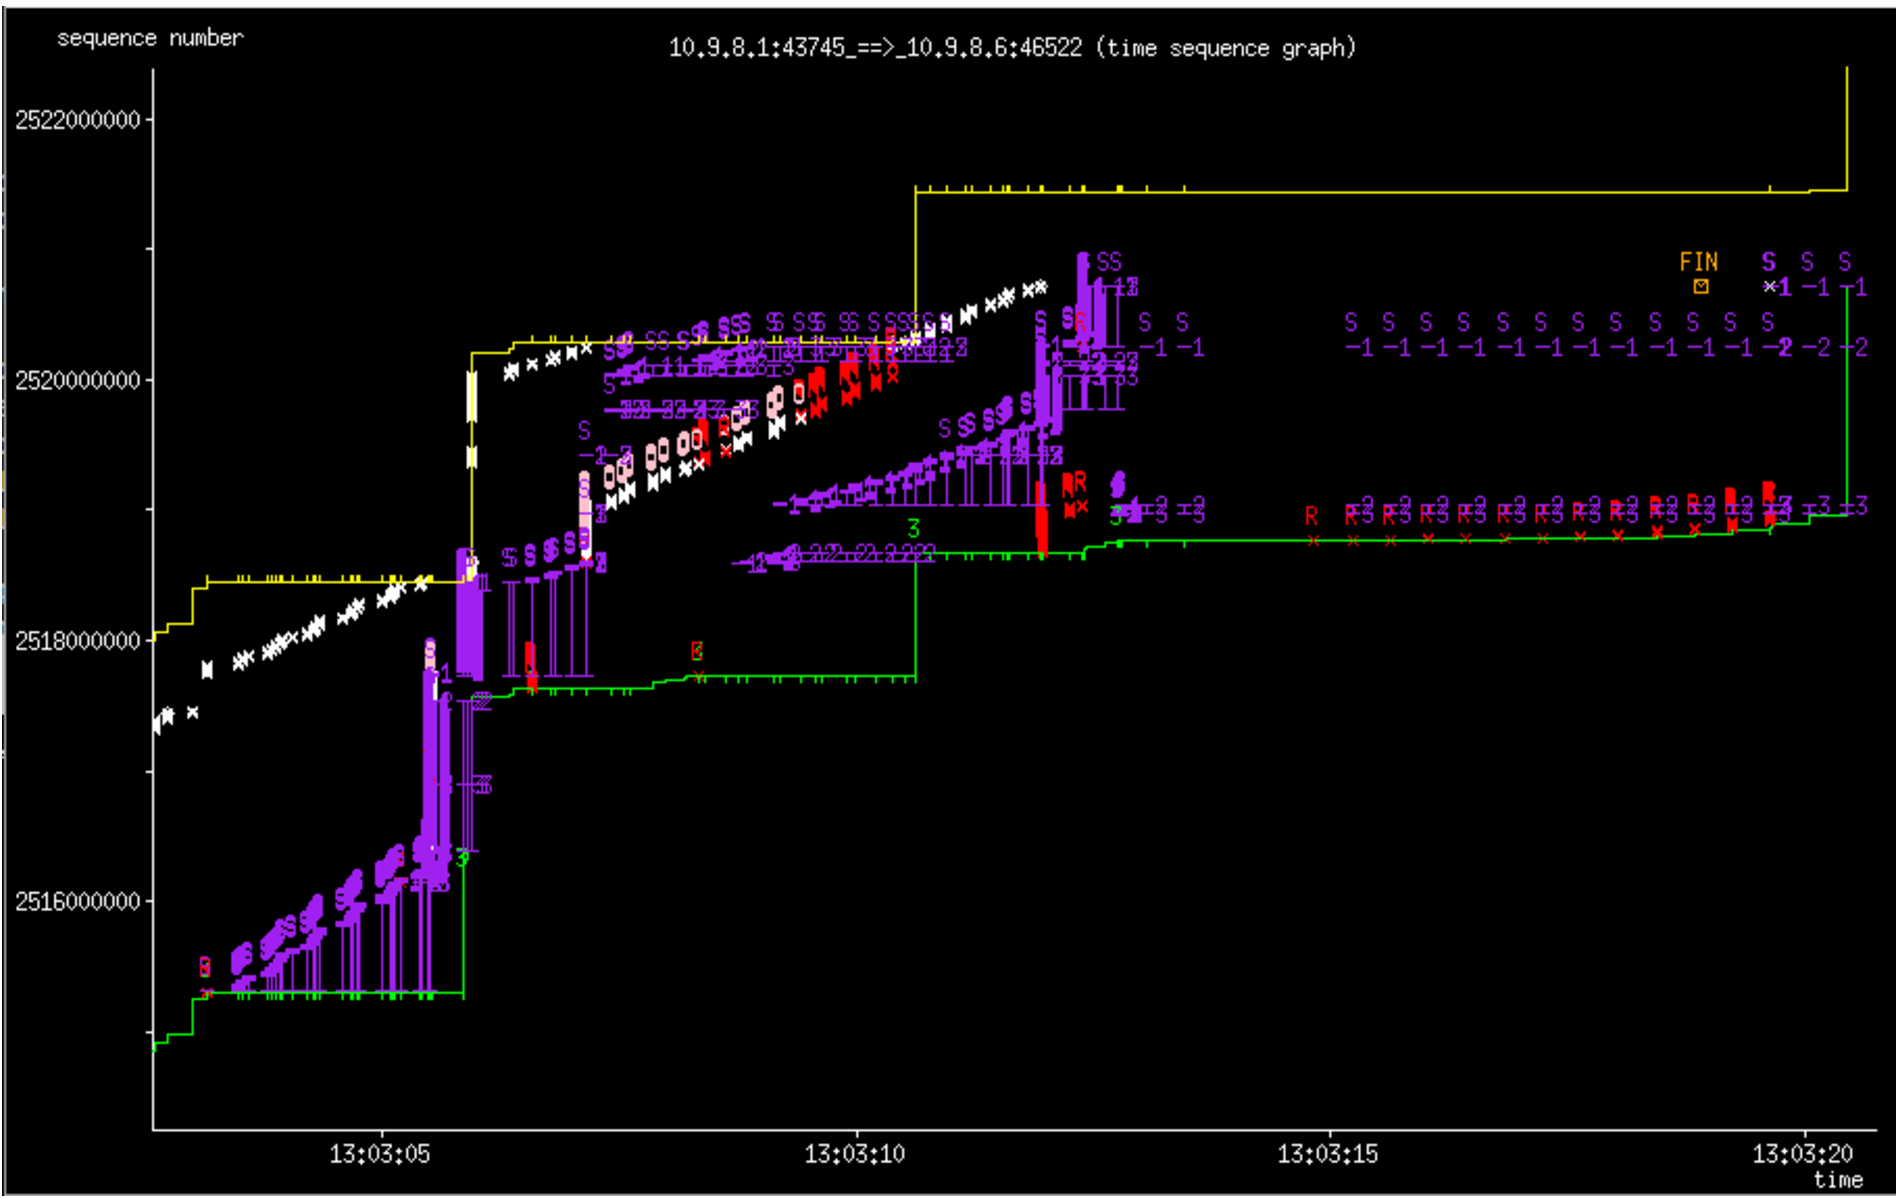
\includegraphics[width=10cm]{../results/lower_layer_seq.pdf}
  \caption{Sequence graph of the lower layer at time 105}
  \label{lower_seq}
\end{figure}

\section{Improving throughput by changing congestion control algorithm} \label{sec:improving_throughput_congestion_control}

In this test I will try switching between different congestion control algorithms, using cubic, lia, olia and wvegas, advised by Olivier Bonaventure and Benjamin Hesmans.

I first take the setup from the first test of section \ref{sec:bulk_data_transfer} to compare the results between the algorithms.

Figure \ref{all_congestion_algo_2rtt} shows that they all give similar results expect wvegas which use both subflow but keep the maximum throughput equivalent to the maximum throughput of only one link.

\begin{figure}[h!]
  \centering
  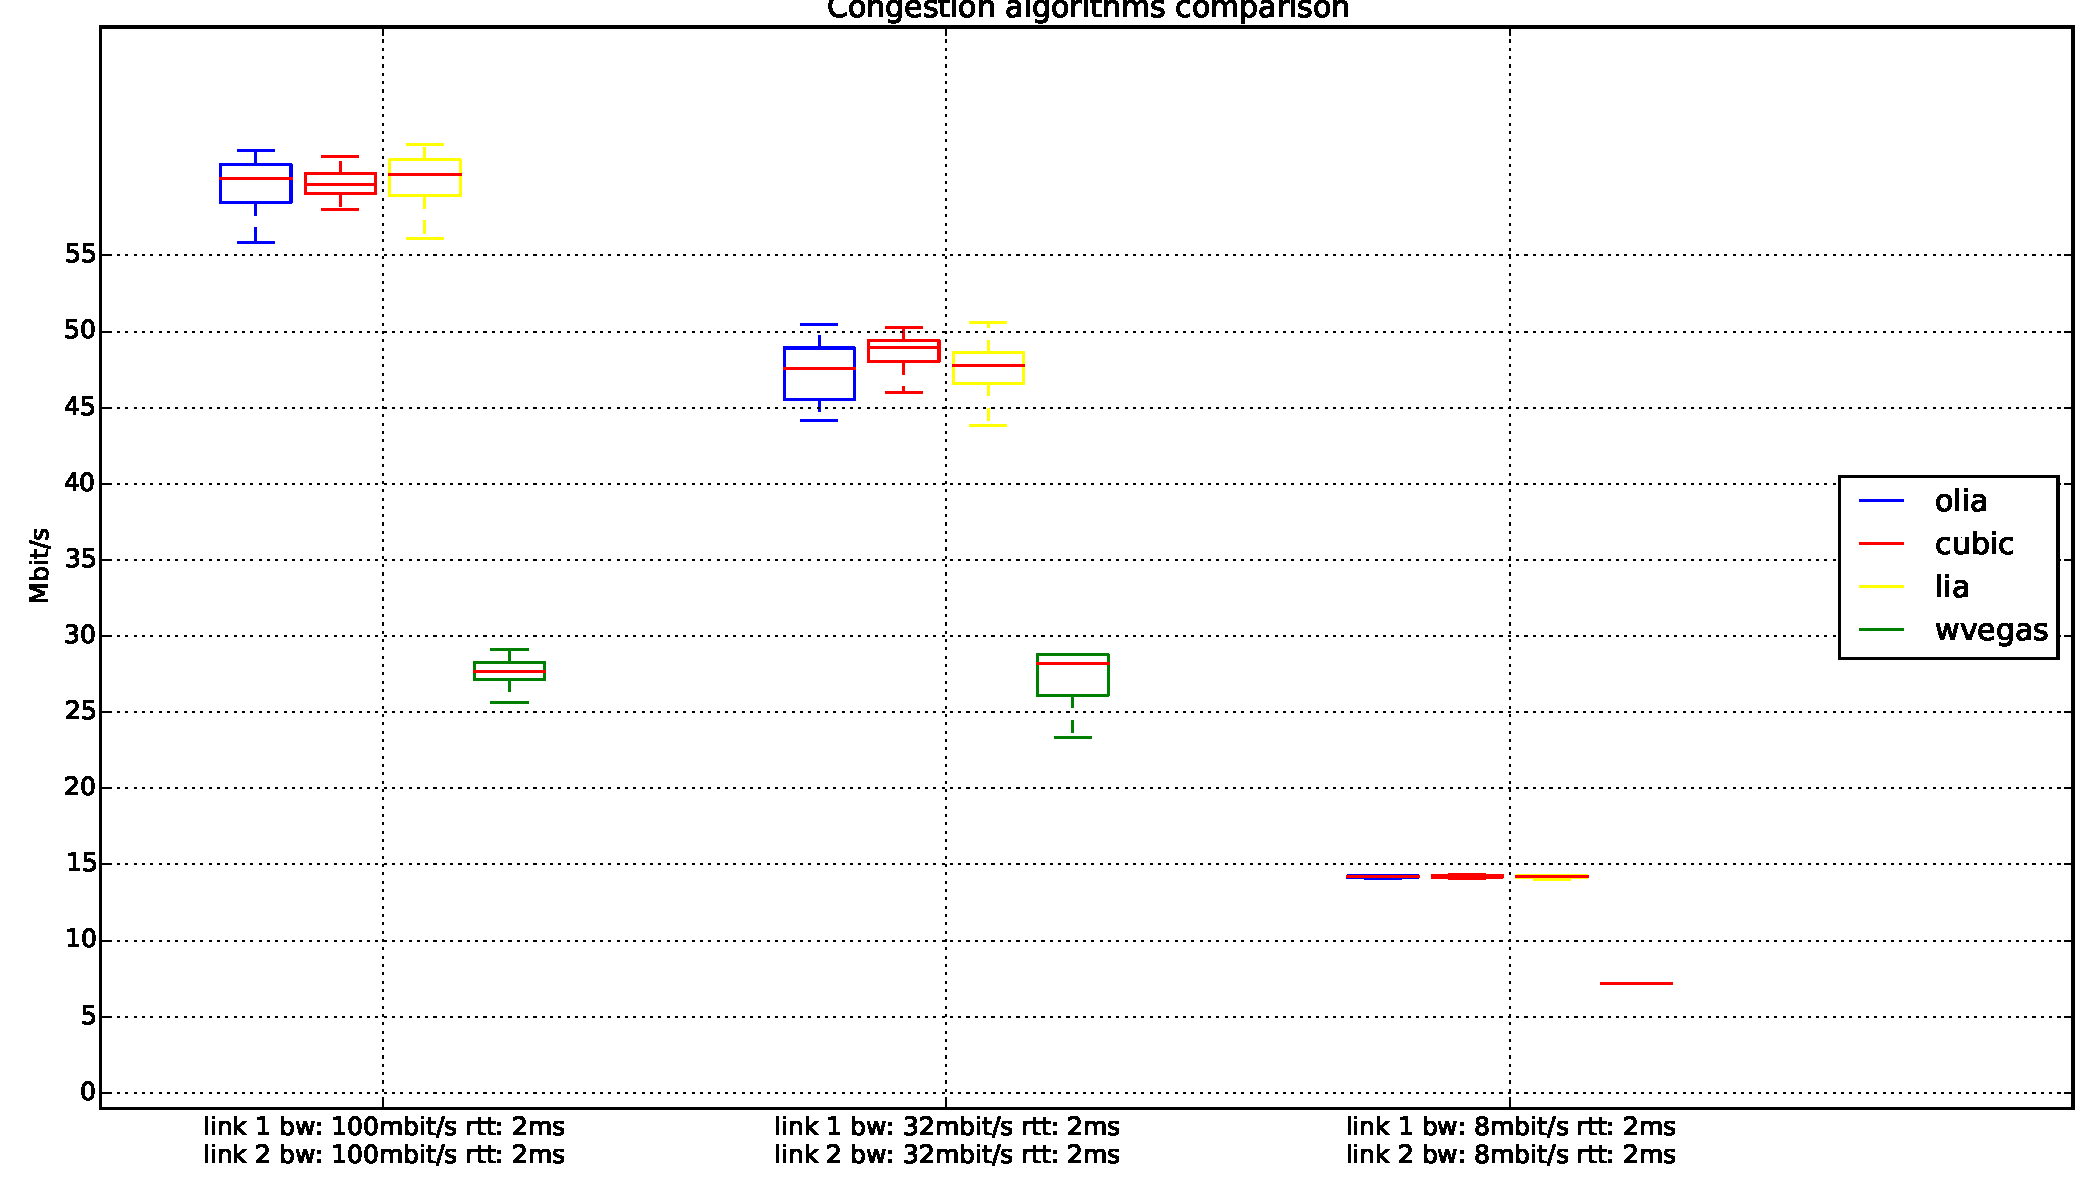
\includegraphics[width=1\textwidth]{../results/all_congestion_algo_2rrt.pdf}
  \caption{Congestion algorithms comparison}
  \label{all_congestion_algo_2rtt}
\end{figure}


Secondly I use setups from test \ref{sec:first_test} and \ref{sec:third_test} to determine wether the algorithms can make a better use of the two subflows when they have different bandwith and RTT.

Figure \ref{all_congestion_algo} show that for setup from section \ref{sec:first_test} the throughput is
almost the same accross all the algorithms except it is a bit lower for wvegas and olia. This is likely due to the fact that they are more fair to normal TCP compared to the others.

For setup from section \ref{sec:third_test}, the wvegas algorithm does not provide a very good throughput.

From paper \cite{cao2012delay}, the autors says that wvegas algorithm is not very efficient with High Delay Bandwith product link.
The cause is the slow start phase of wvegas being very short and switching to congestion avoidance very early.
I tried using a single link with a High delay and High bandwidth and it brought a very low throughput about 100kbit/s on a link with a bandwidth of 32mbit/s and a RTT 400.
Another thing wvegas seems to have a hard time with is link with different RTT, it will usually pick only the link having the lowest RTT and not use the link with the Highest RTT even
if it is not a huge RTT.

To determine what happened with wvegas, I analyzed the capture with MPTCPTrace and TCPTrace. MPTCPTrace showed that both subflow were used but the one with the lowest RTT was used more often.
Another interesting thing is that the TCP windows on the sender side was very small which would explain why we get this very low throughput (see figure \ref{sender_windows_size})

\begin{figure}[h!]
  \centering
  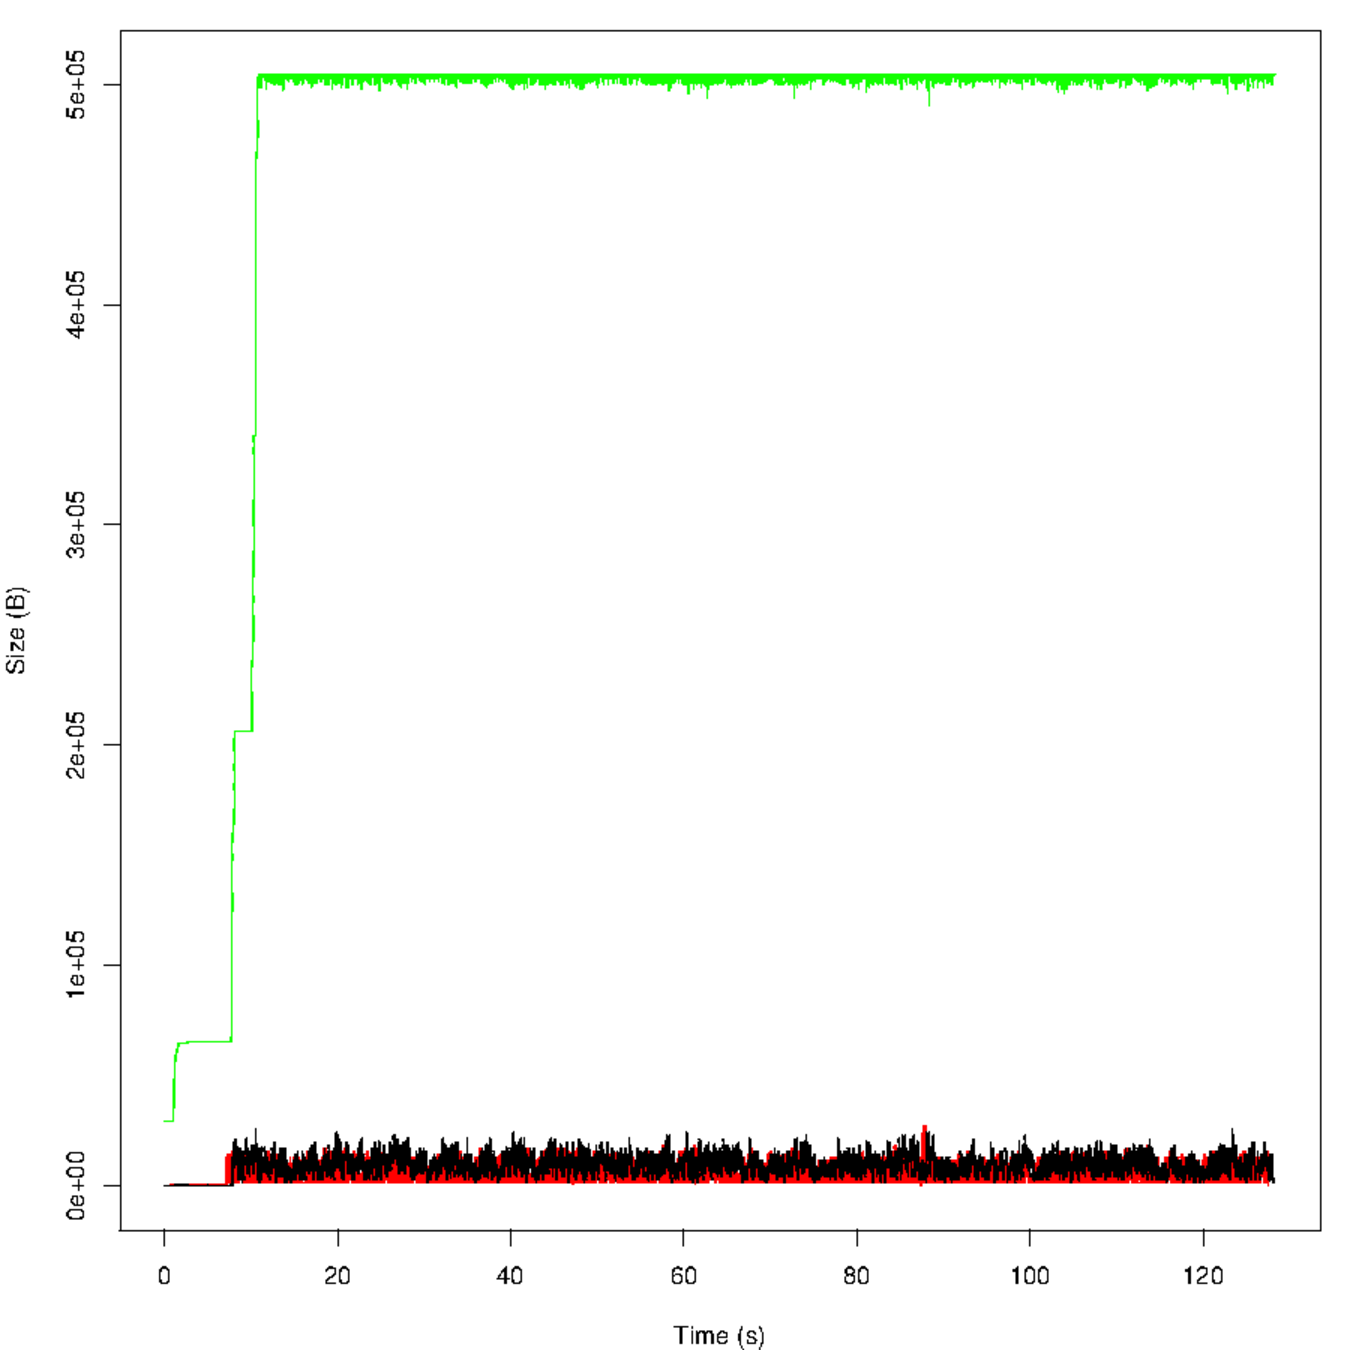
\includegraphics[width=8cm]{../results/window_wvegas_small.pdf}
  \caption{Sender windows size with wVegas}
  \label{sender_windows_size}
\end{figure}

\begin{figure}[h!]
  \centering
  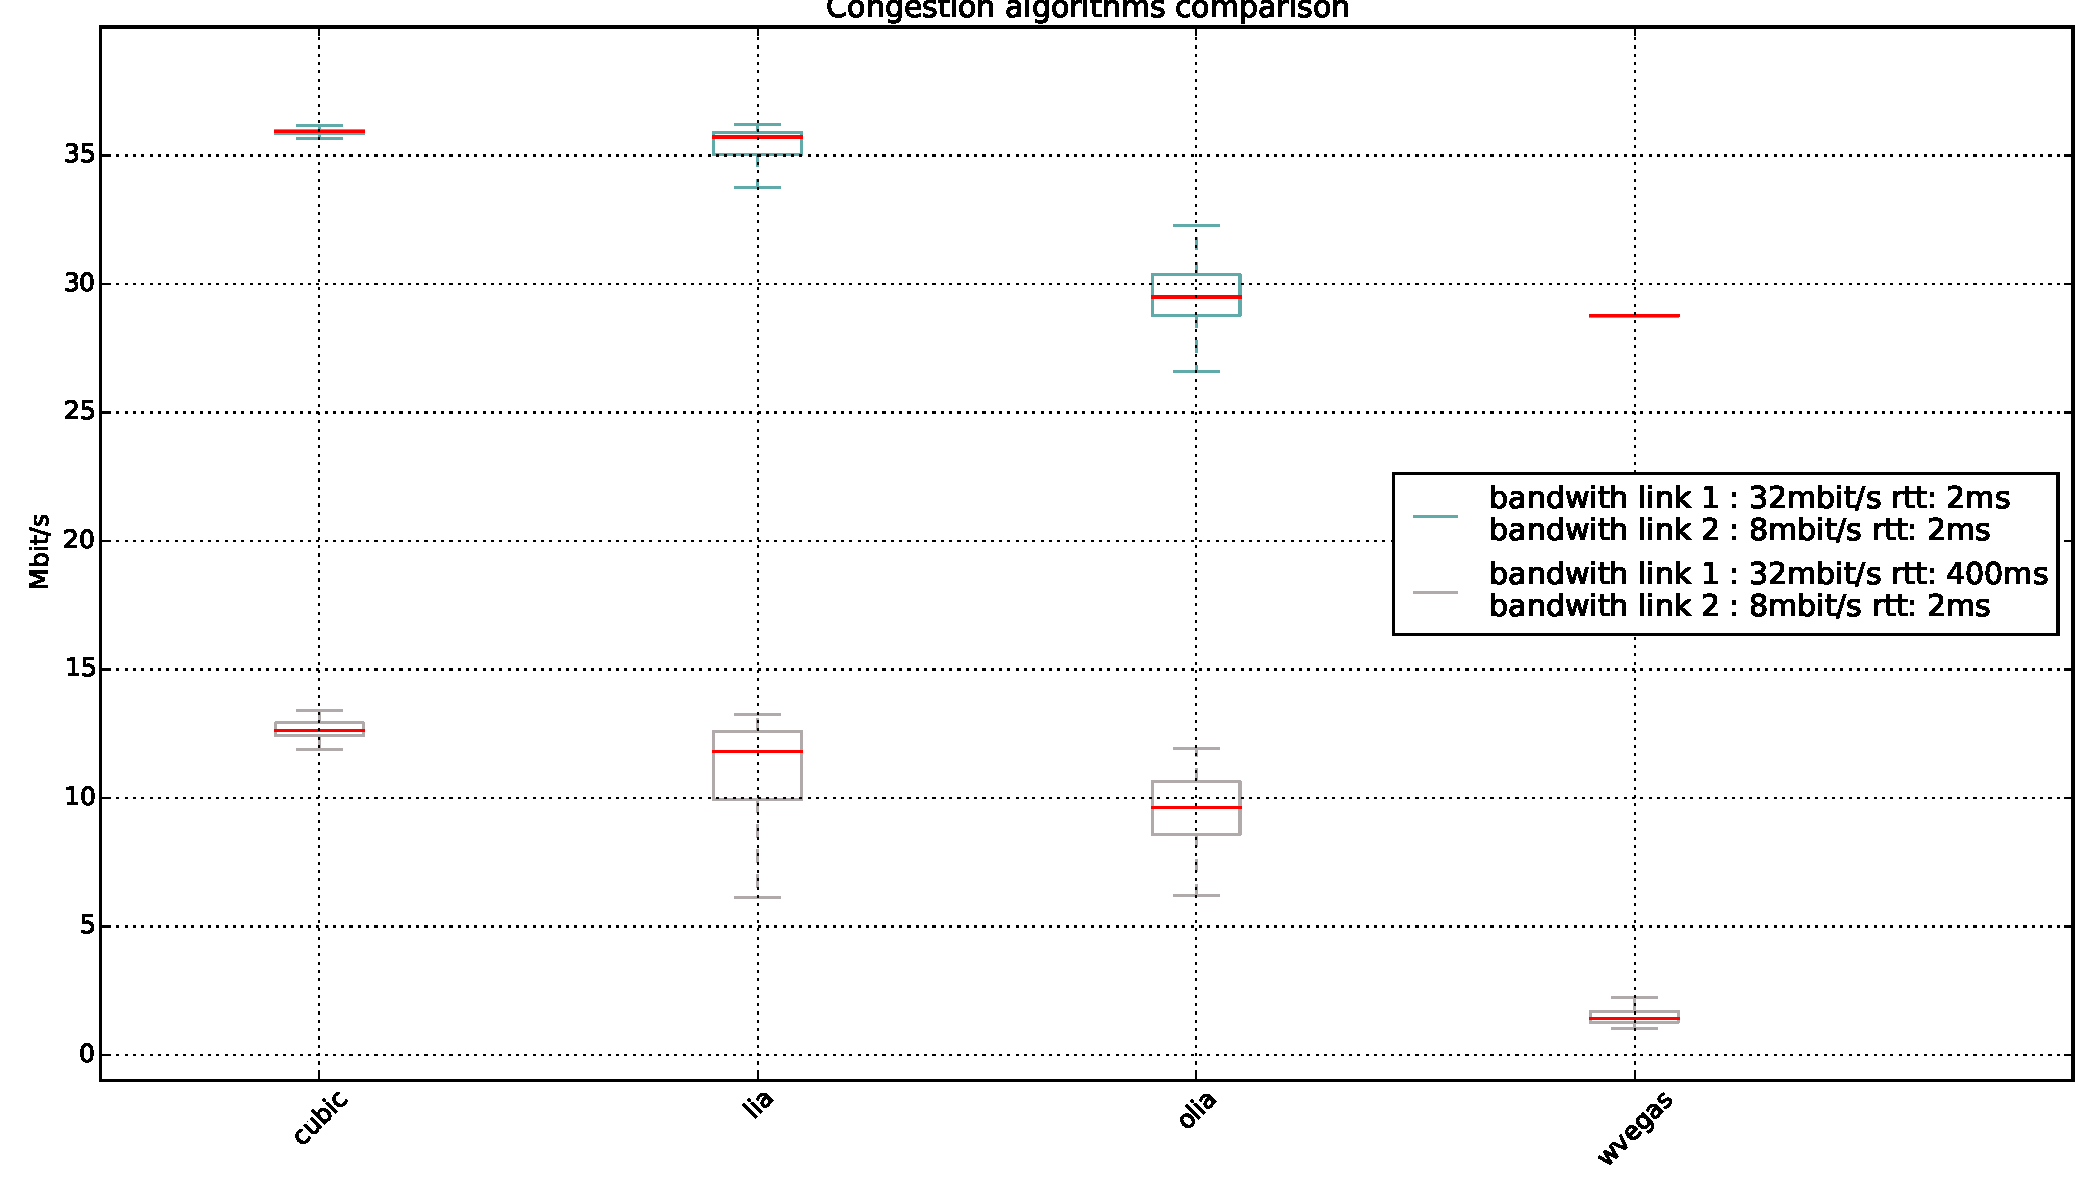
\includegraphics[width=1\textwidth]{../results/all_congestion_algo.pdf}
  \caption{Congestion algorithms comparison}
  \label{all_congestion_algo}
\end{figure}

\newpage

\section{Improving throughput by changing mptcp scheduler} \label{sec:improving_throughput_scheduler}


In test from section \ref{sec:third_test}, we saw that the MPTCP scheduler choose the subflow with the lowest RTT and from time to time use the subflow with the high RTT.
In this section I try to force MPTCP to use the High RTT subflow.

In this purpose I will change the MPTCP scheduler to Roundrobin and look at the effect on the overall throughput.
Roundrobin scheduler does not select subflow based on the RTT, it uses each subflow one after the other
(see section \ref{sec:mptcp_exp} for more information). The expectation is thus that the link with a high RTT will be used and the throughput will increase.

The RoundRobin will use $1$ as the \textit{num\_segments} parameter, number of consecutive segments that should be sent on one subflow and the parameter \textit{cwnd\_limited} will be set to \textit{true}
, the default value. The scheduler tries to fill the congestion window on all subflows.

The throughput with roundrobin is around 14mbit/s. Figure \ref{roundrobin} shows how the traffic was split across the two subflows. 

\begin{figure}[h!]
  \centering
  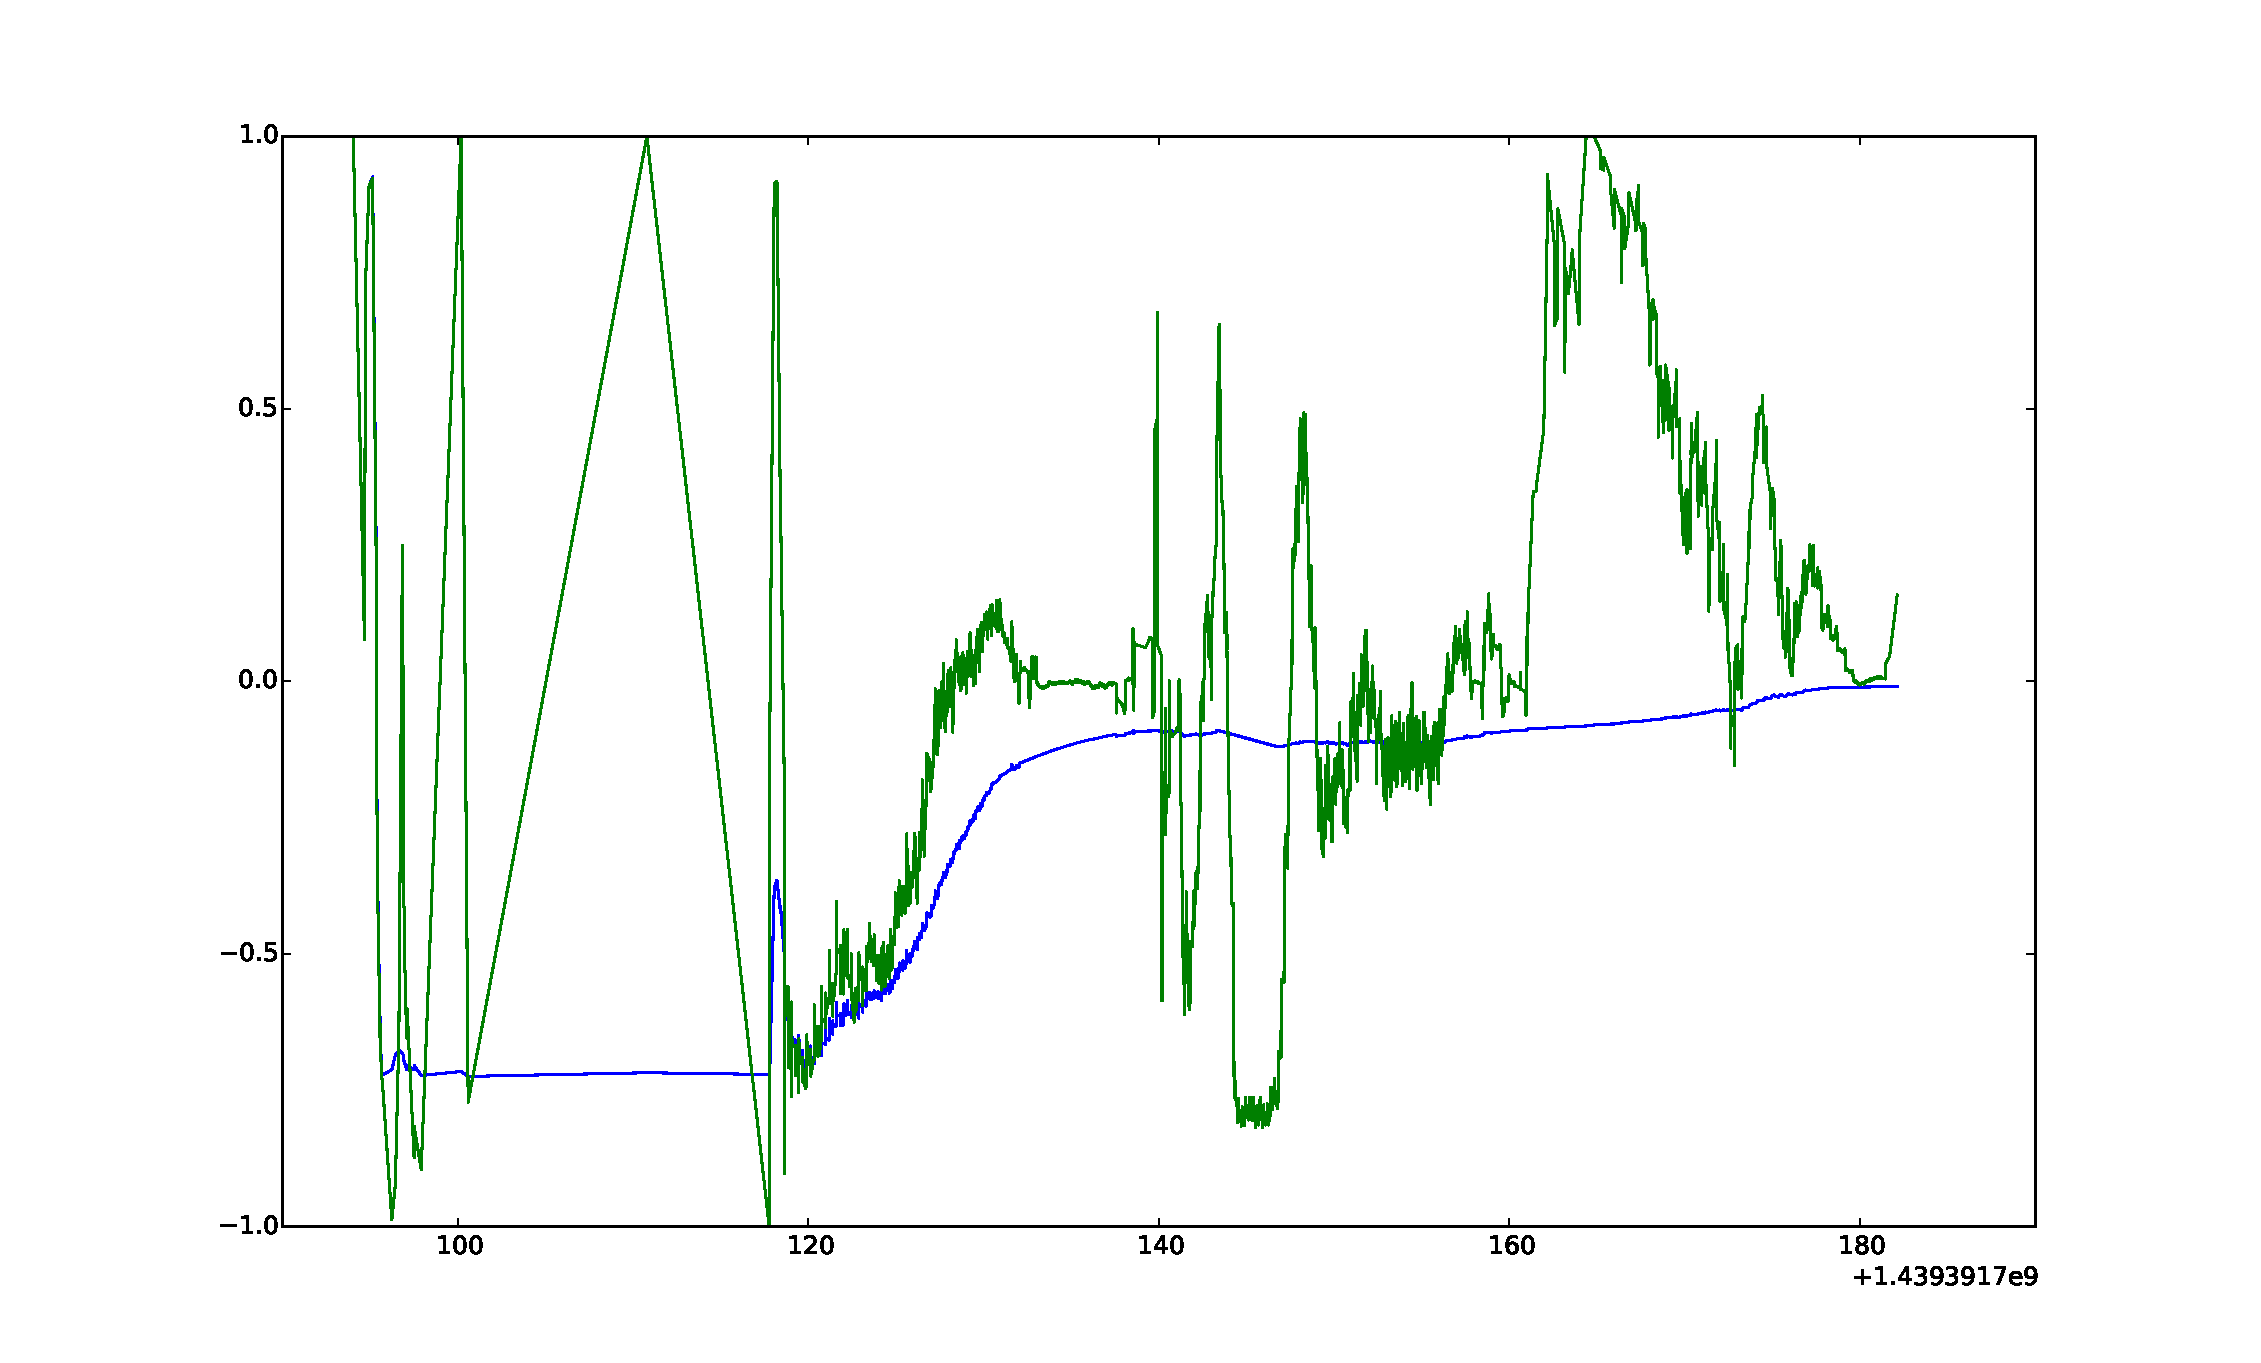
\includegraphics[width=1\textwidth]{../results/roundrobin.pdf}
  \caption{Roundrobin scheduler}
  \label{roundrobin}
\end{figure}
